% ============================================================
%  History of Celestial Mechanics — Beamer Presentation
% ============================================================
%  Compile:  pdflatex lecture_slides.tex
%  Present:  pdfpc lecture_slides.pdf   (Linux/Mac)
%            or open in Adobe Acrobat   (Windows)
%
%  Videos are embedded via \movie (multimedia package).
%  Click the play button on video slides to launch them.
%
%  Required images (optional — placeholders shown if absent):
%    images/ptolemaic_system.jpg
%    images/copernicus.jpg
%
%  Video root path (adjust if your media/ is elsewhere):
\newcommand{\videoroot}{../../media/videos}
\newcommand{\vq}{480p15}   % 480p15 | 720p30 | 1080p60
% ============================================================

\documentclass[aspectratio=169, 14pt]{beamer}

% ── Packages ───────────────────────────────────────────────
\usepackage[utf8]{inputenc}
\usepackage[T2A]{fontenc}
\usepackage[english]{babel}
\usepackage{amsmath, amssymb}
\usepackage{graphicx}
\usepackage{multimedia}          % \movie command
\usepackage{tikz}
\usepackage{hyperref}
\usepackage{color}
\usepackage{amsopn}

% ── Dark astronomy theme ──────────────────────────────────
\usetheme{default}
\setbeamertemplate{navigation symbols}{}
\setbeamertemplate{footline}{%
  \hfill{\color{dimtext}\tiny\insertframenumber}\hspace{4pt}\vspace{3pt}}

\definecolor{darkbg}{RGB}{12, 12, 24}
\definecolor{lighttext}{RGB}{215, 215, 225}
\definecolor{accent}{RGB}{90, 140, 250}
\definecolor{highlight}{RGB}{255, 200, 50}
\definecolor{dimtext}{RGB}{100, 100, 120}

\setbeamercolor{background canvas}{bg=darkbg}
\setbeamercolor{normal text}{fg=lighttext}
\setbeamercolor{frametitle}{fg=highlight, bg=darkbg}
\setbeamercolor{title}{fg=highlight}
\setbeamercolor{subtitle}{fg=accent}
\setbeamercolor{item}{fg=accent}
\setbeamercolor{block title}{fg=highlight, bg=darkbg!80!black}
\setbeamercolor{block body}{fg=lighttext, bg=darkbg!60!black}

\setbeamerfont{frametitle}{size=\Large, series=\bfseries}
\setbeamerfont{title}{size=\huge, series=\bfseries}

% ── Macros ─────────────────────────────────────────────────

% Video play-button slide
\newcommand{\playvideo}[3]{% {display title}{script dir}{scene class}
  \begin{center}
    \movie[width=0.82\linewidth, height=0.461\linewidth, externalviewer]%
    {\fcolorbox{accent}{darkbg!80!black}{%
      \parbox{0.78\linewidth}{\centering\vspace{0.9cm}%
        {\color{accent}\fontsize{48}{48}\selectfont $\blacktriangleright$}\\[10pt]%
        {\color{lighttext}\large #1}\\[6pt]%
        {\color{dimtext}\small Click to play}%
      \vspace{0.9cm}}}}%
    {\videoroot/#2/\vq/#3.mp4}%
  \end{center}
}

% Image with graceful fallback when file is missing
\newcommand{\optimage}[3][width=0.5\linewidth]{%
  \IfFileExists{#2}%
    {\includegraphics[#1]{#2}}%
    {\fcolorbox{accent}{darkbg!80!black}{%
      \parbox{0.38\linewidth}{\centering\vspace{0.4cm}%
        {\color{dimtext}\small #3}\vspace{0.4cm}}}}%
}

% ── Title data ─────────────────────────────────────────────
\title{History of Celestial Mechanics}
\subtitle{From Ptolemy to Satellite Constellations}
\date{}
\author{}

% ============================================================
\begin{document}
% ============================================================


% ━━━━━━━━━━━━━━━━━━━━━━━━━━━━━━━━━━━━━━━━━━━━━━━━━━━━━━━━━━
%  TITLE SLIDE
% ━━━━━━━━━━━━━━━━━━━━━━━━━━━━━━━━━━━━━━━━━━━━━━━━━━━━━━━━━━
\begin{frame}[plain]
  \vfill
  \begin{center}
    {\usebeamerfont{title}\usebeamercolor[fg]{title}\inserttitle}\\[14pt]
    {\usebeamerfont{subtitle}\usebeamercolor[fg]{subtitle}\insertsubtitle}
  \end{center}
  \vfill
  \begin{center}
    {\color{dimtext}\small Press $\rightarrow$ to advance}
  \end{center}
  \vfill
\end{frame}


% ━━━━━━━━━━━━━━━━━━━━━━━━━━━━━━━━━━━━━━━━━━━━━━━━━━━━━━━━━━
%  HISTORICAL TIMELINE
% ━━━━━━━━━━━━━━━━━━━━━━━━━━━━━━━━━━━━━━━━━━━━━━━━━━━━━━━━━━
\begin{frame}{Historical Timeline}
  \vfill
  \begin{center}
    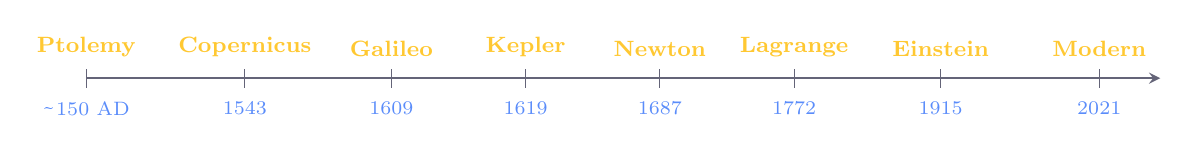
\begin{tikzpicture}[x=1.55cm, y=1cm]
      % Main timeline axis
      \draw[dimtext, thick] (0,0) -- (8.5,0);
      % Tick marks and labels
      \foreach \x/\name/\yr in {
        0/Ptolemy/{\raise2pt\hbox{\texttildelow}}150 AD,
        1.3/Copernicus/1543,
        2.5/Galileo/1609,
        3.6/Kepler/1619,
        4.7/Newton/1687,
        5.8/Lagrange/1772,
        7.0/Einstein/1915,
        8.3/Modern/2021%
      }{
        \draw[dimtext] (\x, -0.12) -- (\x, 0.12);
        \node[above, highlight, font=\footnotesize\bfseries] at (\x, 0.15) {\name};
        \node[below, accent, font=\scriptsize] at (\x, -0.18) {\yr};
      }
      % Arrowheads
      \draw[dimtext, thick, -stealth] (8.5,0) -- (8.8,0);
    \end{tikzpicture}
  \end{center}
  \vfill
\end{frame}


% ━━━━━━━━━━━━━━━━━━━━━━━━━━━━━━━━━━━━━━━━━━━━━━━━━━━━━━━━━━
%  SECTION 1: PTOLEMY & EPICYCLES
% ━━━━━━━━━━━━━━━━━━━━━━━━━━━━━━━━━━━━━━━━━━━━━━━━━━━━━━━━━━

\begin{frame}{The Ptolemaic Universe}
  \begin{columns}[T]
    \column{0.48\linewidth}
    \begin{center}
      \optimage[width=0.88\linewidth]{images/ptolemaic_system.jpg}{%
        Image placeholder:\\[4pt]
        Ptolemaic geocentric model\\[4pt]
        {\footnotesize\texttt{images/ptolemaic\_system.jpg}}}
    \end{center}
    \column{0.52\linewidth}
    \begin{itemize}
      \item Earth at the center of the universe
      \item Planets move on \textbf{epicycles}\\
            (circles upon circles)
      \item Explained retrograde motion
      \item Dominated astronomy for \textbf{1400 years}
    \end{itemize}
    \vspace{8pt}
    \begin{center}
      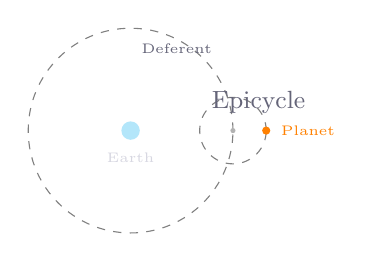
\begin{tikzpicture}[scale=0.65]
        \fill[cyan!30] (0,0) circle (0.18);
        \node[lighttext, font=\tiny, below] at (0,-0.25) {Earth};
        \draw[gray, dashed] (0,0) circle (2.0);
        \node[dimtext, font=\tiny] at (0.9,1.6) {Deferent};
        \fill[gray!60] (2,0) circle (0.05);
        \draw[gray, dashed] (2,0) circle (0.65);
        \node[dimtext, font=\tiny] at (2.5,0.55) {\small Epicycle};
        \fill[orange] (2.65,0) circle (0.08);
        \node[orange, font=\tiny, right] at (2.75,0) {Planet};
      \end{tikzpicture}
    \end{center}
  \end{columns}
\end{frame}


\begin{frame}{Copernicus: The Heliocentric Revolution}
  \begin{columns}[T]
    \column{0.42\linewidth}
    \begin{center}
      \optimage[width=0.85\linewidth]{images/copernicus.jpg}{%
        Portrait placeholder:\\[4pt]
        Nicolaus Copernicus\\(1473--1543)\\[4pt]
        {\footnotesize\texttt{images/copernicus.jpg}}}
    \end{center}
    \column{0.58\linewidth}
    \begin{itemize}
      \item Sun at the center
      \item Simpler explanation of retrograde motion
      \item \textit{De Revolutionibus} (1543)
      \item Still used circular orbits!
    \end{itemize}
    \vspace{8pt}
    \begin{center}
      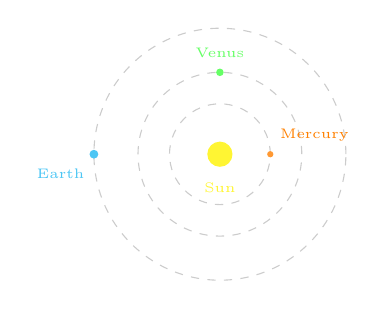
\begin{tikzpicture}[scale=0.8]
        \fill[yellow!80] (0,0) circle (0.2);
        \node[yellow!80, font=\tiny, below] at (0,-0.3) {Sun};
        \draw[gray!40, dashed] (0,0) circle (0.8);
        \draw[gray!40, dashed] (0,0) circle (1.3);
        \draw[gray!40, dashed] (0,0) circle (2.0);
        \fill[orange!80] (0.8,0) circle (0.05);
        \node[orange, font=\tiny, above right] at (0.8,0.05) {Mercury};
        \fill[green!60] (0,1.3) circle (0.06);
        \node[green!60, font=\tiny, above] at (0,1.38) {Venus};
        \fill[cyan!70] (-2.0,0) circle (0.07);
        \node[cyan!70, font=\tiny, below left] at (-2.0,-0.08) {Earth};
      \end{tikzpicture}
    \end{center}
  \end{columns}
\end{frame}


% ── Retrograde Motion ─────────────────────────────────────
\begin{frame}{What is Retrograde Motion?}
  \begin{columns}[T]
    \column{0.50\linewidth}
    \begin{itemize}
      \item Planets sometimes appear to move \textbf{backward}
            against the background stars
      \item The word \textit{planet} comes from the Greek
            \textit{plan\={e}t\={e}s} --- ``\textbf{wanderer}''
      \item Caused by Earth overtaking (or being overtaken by)
            another planet in its orbit
    \end{itemize}

    \column{0.50\linewidth}
    \begin{center}
      {\small\color{accent} Apparent path of Mars on the sky}\\[8pt]
      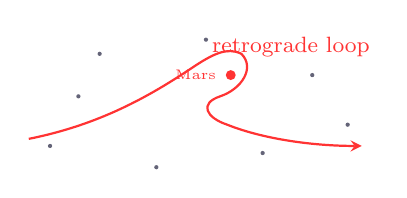
\begin{tikzpicture}[scale=0.9]
        % Background star field dots
        \foreach \sx/\sy in {-0.5/1.8, 1.0/2.0, 2.5/1.5, -1.2/0.5,
                             3.0/0.8, 0.3/0.2, 1.8/0.4, -0.8/1.2}{
          \fill[dimtext] (\sx,\sy) circle (0.03);
        }
        % S-shaped retrograde loop for Mars
        \draw[red!80, thick, -stealth]
          (-1.5, 0.6)
          .. controls (-0.5, 0.8) and (0.2, 1.2) ..
          (0.8, 1.6)
          .. controls (1.1, 1.8) and (1.3, 1.9) ..
          (1.5, 1.8)        % top of loop
          .. controls (1.7, 1.6) and (1.5, 1.3) ..
          (1.2, 1.2)        % bottom of loop (retrograde)
          .. controls (0.9, 1.1) and (1.0, 0.9) ..
          (1.3, 0.8)
          .. controls (1.8, 0.6) and (2.5, 0.5) ..
          (3.2, 0.5);
        % Label
        \node[red!80, font=\footnotesize] at (2.2, 1.9) {retrograde loop};
        \fill[red!80] (1.35, 1.5) circle (0.07);
        \node[red!80, font=\tiny, left] at (1.28, 1.5) {Mars};
      \end{tikzpicture}
    \end{center}
  \end{columns}
\end{frame}


\begin{frame}{Animation: Retrograde Motion}
  \playvideo{Retrograde Motion}{retrograde\_motion}{RetrogradeMotionScene}
\end{frame}


% ── Key Insight: Retrograde ───────────────────────────────
\begin{frame}[plain]
  \vfill
  \begin{center}
    \fcolorbox{highlight}{darkbg!80!black}{%
      \parbox{0.75\linewidth}{\centering\vspace{8pt}%
        {\color{highlight}\large Key Insight}\\[8pt]%
        {\color{lighttext} Both geocentric and heliocentric models explain retrograde motion. But the heliocentric model is far simpler --- Occam's razor at work.}%
      \vspace{8pt}}}
  \end{center}
  \vfill
\end{frame}


\begin{frame}{Epicycles $=$ Fourier Series}
  Any closed curve can be decomposed into circular motions:
  \vspace{6pt}
  \[
    z(\theta) \;=\; \sum_{n=-N}^{N} c_n \, e^{\,i\, n\, \theta}
  \]
  \vspace{2pt}

  \pause
  Each term $c_n \, e^{\,i n \theta}$ is a \textbf{uniform circular motion}:
  \begin{itemize}
    \item Radius $= |c_n|$ \quad {\color{dimtext}(size of the epicycle)}
    \item Angular velocity $= n$ \quad {\color{dimtext}(integer revolutions)}
    \item Initial phase $= \arg(c_n)$
  \end{itemize}

  \pause
  \vspace{10pt}
  \begin{center}
    \fcolorbox{highlight}{darkbg!80!black}{%
      \parbox{0.7\linewidth}{\centering\vspace{4pt}%
        {\color{highlight} Ptolemy's epicycles are a truncated Fourier series!}%
      \vspace{4pt}}}
  \end{center}
\end{frame}


\begin{frame}{Animation: Epicycles \& Fourier Reconstruction}
  \playvideo{Ptolemy's Epicycles}{epicycles}{EpicycleScene}
\end{frame}


% ── Key Insight: Epicycles ────────────────────────────────
\begin{frame}[plain]
  \vfill
  \begin{center}
    \fcolorbox{highlight}{darkbg!80!black}{%
      \parbox{0.75\linewidth}{\centering\vspace{8pt}%
        {\color{highlight}\large Key Insight}\\[8pt]%
        {\color{lighttext} Ptolemy's epicycles are a truncated Fourier series. Any periodic motion can be decomposed into a sum of uniform circular motions.}%
      \vspace{8pt}}}
  \end{center}
  \vfill
\end{frame}


% ━━━━━━━━━━━━━━━━━━━━━━━━━━━━━━━━━━━━━━━━━━━━━━━━━━━━━━━━━━
%  SECTION 2: GALILEO
% ━━━━━━━━━━━━━━━━━━━━━━━━━━━━━━━━━━━━━━━━━━━━━━━━━━━━━━━━━━

\begin{frame}{Galileo: Projectile Motion}
  \begin{columns}[T]
    \column{0.5\linewidth}
    Horizontal and vertical motions are \textbf{independent}:
    \begin{align*}
      x(t) &= v_0 \cos\theta \cdot t \\[6pt]
      y(t) &= v_0 \sin\theta \cdot t - \tfrac{1}{2}\,g\,t^2
    \end{align*}
    \column{0.5\linewidth}
    Eliminate $t$:
    \[
      \boxed{\;y = x\tan\theta - \frac{g\,x^2}{2\,v_0^2\cos^2\!\theta}\;}
    \]
    \vspace{6pt}
    {\color{accent}$\Rightarrow$ This is a \textbf{parabola!}}

    \vspace{12pt}
    Maximum range at $\theta = 45^\circ$:
    \[
      R_{\max} = \frac{v_0^2}{g}
    \]
  \end{columns}
\end{frame}


\begin{frame}{Animation: Projectile Trajectories}
  \playvideo{Galileo: Projectile Motion}{galileo\_projectile}{GalileoProjectileScene}
\end{frame}


% ── Key Insight: Galileo ──────────────────────────────────
\begin{frame}[plain]
  \vfill
  \begin{center}
    \fcolorbox{highlight}{darkbg!80!black}{%
      \parbox{0.75\linewidth}{\centering\vspace{8pt}%
        {\color{highlight}\large Key Insight}\\[8pt]%
        {\color{lighttext} Horizontal and vertical motions are independent. This single principle gives us the parabolic trajectory.}%
      \vspace{8pt}}}
  \end{center}
  \vfill
\end{frame}


% ━━━━━━━━━━━━━━━━━━━━━━━━━━━━━━━━━━━━━━━━━━━━━━━━━━━━━━━━━━
%  SECTION 3: KEPLER
% ━━━━━━━━━━━━━━━━━━━━━━━━━━━━━━━━━━━━━━━━━━━━━━━━━━━━━━━━━━

\begin{frame}{Kepler's Three Laws}
  \textbf{Law 1} --- Orbits are \textbf{ellipses}, Sun at one focus:
  \[
    r(\theta) = \frac{a\,(1-e^2)}{1 + e\cos\theta}
  \]

  \pause
  \textbf{Law 2} --- Equal areas swept in equal times:
  \[
    \frac{dA}{dt} = \frac{L}{2m} = \mathrm{const}
  \]

  \pause
  \textbf{Law 3} --- Orbital period vs.\ semi-major axis:
  \[
    T^2 = \frac{4\pi^2}{GM}\,a^3
  \]
\end{frame}


\begin{frame}{Animation: Kepler's Laws}
  \playvideo{Kepler's Laws}{kepler\_laws}{KeplerLawsScene}
\end{frame}


% ── Key Insight: Kepler ───────────────────────────────────
\begin{frame}[plain]
  \vfill
  \begin{center}
    \fcolorbox{highlight}{darkbg!80!black}{%
      \parbox{0.75\linewidth}{\centering\vspace{8pt}%
        {\color{highlight}\large Key Insight}\\[8pt]%
        {\color{lighttext} Kepler's laws are purely empirical --- he found patterns in data, but had no explanation for \textit{why} orbits are ellipses.}%
      \vspace{8pt}}}
  \end{center}
  \vfill
\end{frame}


% ━━━━━━━━━━━━━━━━━━━━━━━━━━━━━━━━━━━━━━━━━━━━━━━━━━━━━━━━━━
%  SECTION 4: NEWTON
% ━━━━━━━━━━━━━━━━━━━━━━━━━━━━━━━━━━━━━━━━━━━━━━━━━━━━━━━━━━

\begin{frame}{Newton's Universal Gravitation}
  \textbf{The gravitational force:}
  \[
    \vec{F} = -\frac{G\,M\,m}{r^2}\,\hat{r}
  \]

  \pause
  \textbf{Equation of motion:}
  \[
    \ddot{\vec{r}} = -\frac{GM}{|\vec{r}|^3}\,\vec{r}
  \]

  \pause
  \textbf{Binet equation} (polar coordinates, $u = 1/r$):
  \[
    \frac{d^2 u}{d\theta^2} + u = \frac{GM}{L^2}
  \]

  \vspace{4pt}
  Solution: \textbf{conic sections} --- ellipse, parabola, or hyperbola.
\end{frame}


\begin{frame}{Newton's Cannon: From Fall to Orbit}
  \begin{center}
    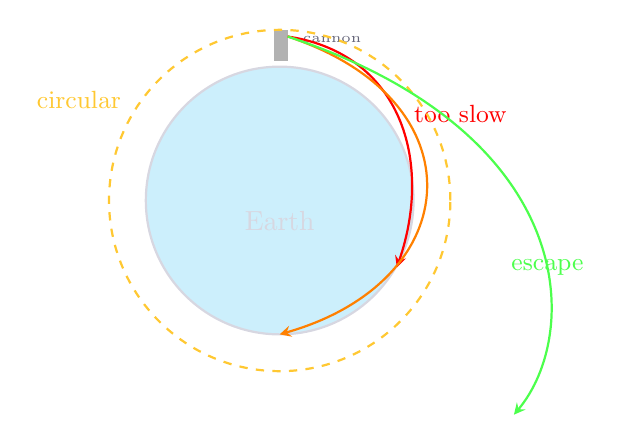
\begin{tikzpicture}[scale=0.85]
      % Earth
      \fill[cyan!20] (0,0) circle (2);
      \draw[lighttext, thick] (0,0) circle (2);
      \node[lighttext] at (0,-0.3) {Earth};
      % cannon
      \fill[gray!60] (-0.08,2.08) rectangle (0.12,2.55);
      \node[dimtext, font=\tiny, right] at (0.2,2.4) {cannon};
      % slow (crash)
      \draw[red, thick, -stealth]
        (0.12,2.45) .. controls (1.8,2.2) and (2.3,0.6) .. (1.75,-1.0);
      \node[red, font=\small] at (2.7,1.3) {too slow};
      % suborbital
      \draw[orange, thick, -stealth]
        (0.12,2.45) .. controls (3.0,1.5) and (2.8,-1.2) .. (0,-2);
      % circular orbit
      \draw[highlight, thick, dashed] (0,0) circle (2.55);
      \node[highlight, font=\small] at (-3.0,1.5) {circular};
      % escape
      \draw[green!70, thick, -stealth]
        (0.12,2.45) .. controls (4.5,1.0) and (4.5,-2.0) .. (3.5,-3.2);
      \node[green!70, font=\small] at (4.0,-1.0) {escape};
    \end{tikzpicture}
  \end{center}
\end{frame}


\begin{frame}{Animation: Newton's Cannon}
  \playvideo{Newton's Cannon}{newton\_gravity}{NewtonCannonballScene}
\end{frame}


% ── Key Insight: Newton ───────────────────────────────────
\begin{frame}[plain]
  \vfill
  \begin{center}
    \fcolorbox{highlight}{darkbg!80!black}{%
      \parbox{0.75\linewidth}{\centering\vspace{8pt}%
        {\color{highlight}\large Key Insight}\\[8pt]%
        {\color{lighttext} The same force that drops an apple curves a cannonball into orbit. Newton unified terrestrial and celestial mechanics.}%
      \vspace{8pt}}}
  \end{center}
  \vfill
\end{frame}


\begin{frame}{Interactive Demo: Orbital Simulator}
  \begin{center}
    \vspace{0.3cm}
    {\Large\color{highlight} Live orbital mechanics simulation}

    \vspace{18pt}
    \href{https://skychart.astrageek.ru/astra-etudes/orbital-simulator}{%
      \fcolorbox{accent}{darkbg!80!black}{%
        \parbox{0.55\linewidth}{\centering\vspace{0.7cm}%
          {\color{accent}\fontsize{40}{40}\selectfont $\oplus$}\\[10pt]%
          {\color{lighttext}\large Open Orbital Simulator}\\[6pt]%
          {\color{dimtext}\small skychart.astrageek.ru/astra-etudes/orbital-simulator}%
        \vspace{0.7cm}}}}

    \vspace{12pt}
    {\color{dimtext}\small Scan QR or visit URL in your browser}
  \end{center}
\end{frame}


% ━━━━━━━━━━━━━━━━━━━━━━━━━━━━━━━━━━━━━━━━━━━━━━━━━━━━━━━━━━
%  SECTION 5: THREE-BODY PROBLEM
% ━━━━━━━━━━━━━━━━━━━━━━━━━━━━━━━━━━━━━━━━━━━━━━━━━━━━━━━━━━

\begin{frame}{The Three-Body Problem}
  \begin{columns}[T]
    \column{0.55\linewidth}
    \begin{itemize}
      \item Two bodies $\to$ \textbf{exact solution} (Kepler orbits)
      \item Three bodies $\to$ \textbf{no general closed-form solution}
      \item Poincar\'{e} (1890): proof of \textbf{chaotic behavior}
      \item Extreme sensitivity to initial conditions
    \end{itemize}
    \column{0.45\linewidth}
    \begin{center}
      \textbf{Pythagorean problem}\\[6pt]
      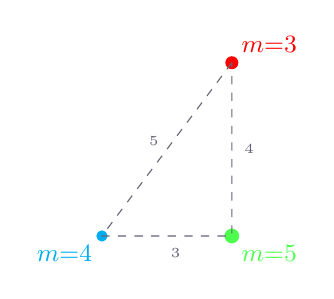
\begin{tikzpicture}[scale=0.55]
        \fill[red] (1,3) circle (0.15) node[above right, font=\small] {$m{=}3$};
        \fill[cyan] (-2,-1) circle (0.13) node[below left, font=\small] {$m{=}4$};
        \fill[green!70] (1,-1) circle (0.17) node[below right, font=\small] {$m{=}5$};
        \draw[dimtext, dashed] (1,3) -- (-2,-1) -- (1,-1) -- cycle;
        \node[dimtext, font=\tiny] at (-0.8,1.2) {5};
        \node[dimtext, font=\tiny] at (-0.3,-1.4) {3};
        \node[dimtext, font=\tiny] at (1.4,1.0) {4};
      \end{tikzpicture}
      \\[6pt]
      {\color{dimtext}\small Masses at rest in a\\3-4-5 right triangle}
    \end{center}
  \end{columns}
\end{frame}


\begin{frame}{Animation: Three-Body Problem}
  \playvideo{Three-Body Problem}{three\_body}{ThreeBodyScene}
\end{frame}


% ── Key Insight: Three-Body ───────────────────────────────
\begin{frame}[plain]
  \vfill
  \begin{center}
    \fcolorbox{highlight}{darkbg!80!black}{%
      \parbox{0.75\linewidth}{\centering\vspace{8pt}%
        {\color{highlight}\large Key Insight}\\[8pt]%
        {\color{lighttext} Adding just one more body destroys exact solvability. The universe is fundamentally chaotic at the three-body level.}%
      \vspace{8pt}}}
  \end{center}
  \vfill
\end{frame}


% ━━━━━━━━━━━━━━━━━━━━━━━━━━━━━━━━━━━━━━━━━━━━━━━━━━━━━━━━━━
%  SECTION 6: LAGRANGE POINTS
% ━━━━━━━━━━━━━━━━━━━━━━━━━━━━━━━━━━━━━━━━━━━━━━━━━━━━━━━━━━

\begin{frame}{Lagrange Points}
  \begin{columns}[T]
    \column{0.50\linewidth}
    In the \textbf{rotating frame} of Sun--Planet:
    \begin{itemize}
      \item 5 equilibrium points (L1--L5)
      \item L1, L2, L3: collinear, \textbf{unstable}
      \item L4, L5: triangular, \textbf{stable}
    \end{itemize}
    \vspace{6pt}
    Jupiter's L4 and L5 host \textbf{Trojan asteroids}\\
    ($>$12\,000 known objects!)

    \column{0.50\linewidth}
    \begin{center}
      \begin{tikzpicture}[scale=1.0]
        \fill[yellow!80] (-0.1,0) circle (0.18);
        \node[yellow!80, font=\tiny, below] at (-0.1,-0.22) {Sun};
        \fill[orange] (2.5,0) circle (0.10);
        \node[orange, font=\tiny, below] at (2.5,-0.15) {Jupiter};
        \draw[gray!30, dashed] (-0.1,0) circle (2.6);
        % Collinear
        \fill[red] (2.0,0) circle (0.05);
        \node[red, font=\tiny, above] at (2.0,0.1) {L1};
        \fill[red] (3.1,0) circle (0.05);
        \node[red, font=\tiny, above] at (3.1,0.1) {L2};
        \fill[red] (-2.7,0) circle (0.05);
        \node[red, font=\tiny, above] at (-2.7,0.1) {L3};
        % Triangular
        \fill[green!80] (1.1,2.15) circle (0.06);
        \node[green!80, font=\tiny, above] at (1.1,2.25) {L4};
        \fill[green!80] (1.1,-2.15) circle (0.06);
        \node[green!80, font=\tiny, below] at (1.1,-2.25) {L5};
        % Dashed equilateral triangles
        \draw[green!50, dashed, thin] (-0.1,0) -- (1.1,2.15) -- (2.5,0);
        \draw[green!50, dashed, thin] (-0.1,0) -- (1.1,-2.15) -- (2.5,0);
      \end{tikzpicture}
    \end{center}
  \end{columns}
\end{frame}


\begin{frame}{Animation: Lagrange Points \& System Rotation}
  \playvideo{Lagrange Points}{lagrange\_points}{LagrangePointsScene}
\end{frame}


% ── Key Insight: Lagrange ─────────────────────────────────
\begin{frame}[plain]
  \vfill
  \begin{center}
    \fcolorbox{highlight}{darkbg!80!black}{%
      \parbox{0.75\linewidth}{\centering\vspace{8pt}%
        {\color{highlight}\large Key Insight}\\[8pt]%
        {\color{lighttext} Equilibrium exists even in a chaotic gravitational landscape. L4 and L5 are stable --- home to thousands of Trojan asteroids.}%
      \vspace{8pt}}}
  \end{center}
  \vfill
\end{frame}


% ━━━━━━━━━━━━━━━━━━━━━━━━━━━━━━━━━━━━━━━━━━━━━━━━━━━━━━━━━━
%  SECTION 7: EINSTEIN & MERCURY
% ━━━━━━━━━━━━━━━━━━━━━━━━━━━━━━━━━━━━━━━━━━━━━━━━━━━━━━━━━━

\begin{frame}{From Newton to Einstein}
  \textbf{Newton's Binet equation:}
  \[
    \frac{d^2 u}{d\theta^2} + u = \frac{GM}{L^2}
    \qquad {\color{dimtext}(u = 1/r)}
  \]

  \pause
  \vspace{8pt}
  \textbf{General Relativity} adds one extra term:
  \[
    \boxed{\;\frac{d^2 u}{d\theta^2} + u
    = \frac{GM}{L^2}
    + \underbrace{\frac{3\,GM}{c^2}\,u^2}_{\text{GR correction}}\;}
  \]

  \pause
  \vspace{8pt}
  This causes \textbf{perihelion precession}:
  \[
    \Delta\varphi
    = \frac{6\pi\,G M}{c^2\,a\,(1-e^2)}
    \quad \text{per orbit}
  \]

  \vspace{4pt}
  \begin{center}
    {\color{highlight} Mercury: $43''$ per century --- confirmed by observation (1915)}
  \end{center}
\end{frame}


\begin{frame}{Animation: Mercury Perihelion Precession}
  \playvideo{Mercury Precession (GR)}{mercury\_precession}{MercuryPrecessionScene}
\end{frame}


% ── Key Insight: Einstein ─────────────────────────────────
\begin{frame}[plain]
  \vfill
  \begin{center}
    \fcolorbox{highlight}{darkbg!80!black}{%
      \parbox{0.75\linewidth}{\centering\vspace{8pt}%
        {\color{highlight}\large Key Insight}\\[8pt]%
        {\color{lighttext} Newton was ``wrong'' --- but only by 43 arcseconds per century. Einstein's tiny correction revealed the curvature of spacetime.}%
      \vspace{8pt}}}
  \end{center}
  \vfill
\end{frame}


% ━━━━━━━━━━━━━━━━━━━━━━━━━━━━━━━━━━━━━━━━━━━━━━━━━━━━━━━━━━
%  MODERN APPLICATIONS
% ━━━━━━━━━━━━━━━━━━━━━━━━━━━━━━━━━━━━━━━━━━━━━━━━━━━━━━━━━━

\begin{frame}{Modern Celestial Mechanics}
  \begin{itemize}
    \item \textbf{JWST} at Sun--Earth L2
          \quad {\color{dimtext}(Lagrange, 1772)}
    \item \textbf{GPS} requires GR time corrections of ${\sim}38\;\mu$s/day
          \quad {\color{dimtext}(Einstein, 1915)}
    \item \textbf{Voyager} gravity assists --- slingshot past Jupiter and Saturn
          \quad {\color{dimtext}(Newton, 1687)}
    \item \textbf{Starlink / OneWeb} constellations ---
          thousands of satellites in low Earth orbit
          \quad {\color{dimtext}(Kepler, 1619)}
  \end{itemize}
  \vspace{10pt}
  \begin{center}
    {\color{accent} Every modern space mission stands on 2000 years of celestial mechanics.}
  \end{center}
\end{frame}


\begin{frame}{Gravity Assists: The Cosmic Slingshot}
  \begin{columns}[T]
    \column{0.50\linewidth}
    \begin{center}
      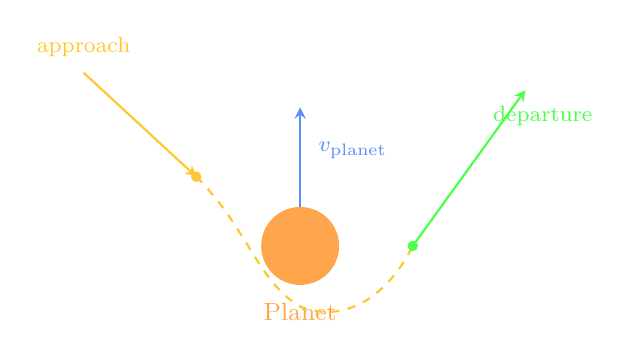
\begin{tikzpicture}[scale=1.1]
        % Planet
        \fill[orange!70] (0,0) circle (0.45);
        \node[orange!70, font=\small, below] at (0,-0.55) {Planet};
        % Planet velocity arrow
        \draw[accent, thick, -stealth] (0,0.45) -- (0,1.6);
        \node[accent, font=\footnotesize, right] at (0.1,1.1) {$v_{\text{planet}}$};
        % Incoming spacecraft
        \draw[highlight, thick, -stealth]
          (-2.5, 2.0) -- (-1.2, 0.8);
        \node[highlight, font=\footnotesize] at (-2.5, 2.3) {approach};
        % Hyperbolic arc around planet
        \draw[highlight, thick, dashed]
          (-1.2, 0.8)
          .. controls (-0.6, 0.2) and (-0.5, -0.4) ..
          (0.0, -0.7)
          .. controls (0.5, -0.9) and (1.0, -0.6) ..
          (1.3, 0.0);
        % Outgoing spacecraft (faster)
        \draw[green!70, thick, -stealth]
          (1.3, 0.0) -- (2.6, 1.8);
        \node[green!70, font=\footnotesize] at (2.8, 1.5) {departure};
        % Spacecraft markers
        \fill[highlight] (-1.2, 0.8) circle (0.06);
        \fill[green!70] (1.3, 0.0) circle (0.06);
      \end{tikzpicture}
    \end{center}

    \column{0.50\linewidth}
    \vspace{10pt}
    In the \textbf{planet's rest frame}, speed is unchanged ---
    the spacecraft merely deflects.

    \vspace{8pt}
    In the \textbf{Sun's frame}, the spacecraft gains up to:
    \[
      \boxed{\;\Delta v = 2\, v_{\text{planet}}\;}
    \]

    \vspace{6pt}
    {\color{dimtext}\small (maximum gain for a $180^\circ$ deflection)}

    \vspace{10pt}
    {\color{accent} Voyager~2 used four gravity assists to reach interstellar space.}
  \end{columns}
\end{frame}


% ━━━━━━━━━━━━━━━━━━━━━━━━━━━━━━━━━━━━━━━━━━━━━━━━━━━━━━━━━━
%  SUMMARY & CLOSING
% ━━━━━━━━━━━━━━━━━━━━━━━━━━━━━━━━━━━━━━━━━━━━━━━━━━━━━━━━━━

\begin{frame}{Summary}
  \begin{center}
    \renewcommand{\arraystretch}{1.5}
    \begin{tabular}{r@{\quad}l}
      {\color{highlight} Ptolemy}   & Epicycles (= Fourier series!) \\
      {\color{highlight} Copernicus}& Heliocentric model \\
      {\color{highlight} Galileo}   & Projectile motion = parabola \\
      {\color{highlight} Kepler}    & Elliptical orbits, three laws \\
      {\color{highlight} Newton}    & Universal gravitation, $F \propto 1/r^2$ \\
      {\color{highlight} Lagrange}  & Equilibrium points L1--L5 \\
      {\color{highlight} Einstein}  & GR correction $\to$ precession \\
    \end{tabular}
  \end{center}

  \vspace{12pt}
  \begin{center}
    {\color{accent}\large From circles to spacetime curvature ---}\\[4pt]
    {\color{accent}\large 2000 years of celestial mechanics}
  \end{center}
\end{frame}


\begin{frame}[plain]
  \vfill
  \begin{center}
    {\fontsize{48}{48}\selectfont\color{highlight} Thank you!}\\[24pt]
    {\color{dimtext}\Large Questions?}
  \end{center}
  \vfill
\end{frame}


\end{document}
